\chapter{Results and discussion}
    \label{chap:results}

\section{Dataset}
    \label{sec:dataset}
    
The data set is made up of 15 3D models, each one representing a different object which has a class in the ImageNet dataset. Each model consists of a 2D texture, a .obj file, and a text file. The .obj file contains the vertices making up the 3D object and each vertex's texture coordinates, while the text file contains a list of correct labels.

All 3D models and their textures were obtained by manually searching 3D asset sites for suitable models, and were not created by me. All credits for the models go to their respective creators, seen in Appendix \ref{app:model_credits}. Each model was manually re-scaled using the Blender 3D graphics tool \footnote{https://www.blender.org/} such that all 15 models are of comparable size. This was done to ensure that each model would not need different rendering parameter distributions to properly fit into the rendered image.

Out of the 15 models, 10 represent the same classes that the dataset of 10 3D models used by Athalye \textit{et al.} \cite{athalye} also represented. This was done in order to properly reproduce the experimental results of Athalye \textit{et al.}. Please keep in mind that these 10 models are not the same ones that Athalye \textit{et al.} used, as they did not publish their dataset. The other 5 models represent other ImageNet classes: a crocodile, a killer whale, a jeep, a running shoe and a rugby ball.

You can view the correct labels for each model in table \ref{table:model_labels_accuracy}, along with the classification accuracy of InceptionV3 on rendered images of each model.

The choice of suitable models was constrained by the following requirements:

\begin{itemize}
    \item The model has to be free.
    \item It has to have a texture, not a solid colour.
    \item It has to have only one texture, not multiple ones for different parts of the object, as the renderer only applies one texture to the object.
    \item Rendered images of the model must be classified accurately by a pre-trained InceptionV3 classifier at least 30\% of the time.
    \item The model must not have transparent surfaces such as car windows, as the implemented renderer can not calculate UV coordinates for that surface.
\end{itemize}

Due to the above requirements, I could not find a very good 3D model for a taxi. The one I settled for has a different texture for its wheels and license plates, and the renderer simply applies parts of the main texture of the body of the taxi to the wheels, making them look yellow, as you can see in figure \ref{fig:taxi}. Similarly, a suitable model for a sofa, as used by Athalye \textit{et al.} \cite{athalye}, could not be found. Several models that I tried were classified correctly by an InceptionV3 classifier less than 10\% of the time. Therefore, a 3D model of a purse is used instead.

\begin{figure}[ht]
    \centering
    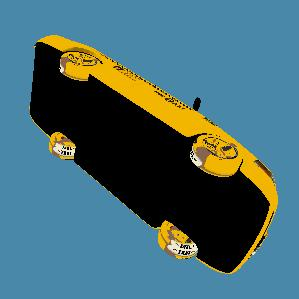
\includegraphics[width=0.4\textwidth]{graphics/taxi.jpg}
    \caption{A render of the taxi model with its normal texture. As you can see, the renderer applies parts of the car body texture to the wheels.}
    \label{fig:taxi}
\end{figure}

The original textures of the model had a resolution of 1024x1024, 2048x2048 or 4096x496 pixels. Since the generator requires each input texture to have the same size, the 4096x4096 textures were downsampled to 2048x2048 using OpenCV's resize function with INTER\_AREA interpolation \footnote{https://learnopencv.com/image-resizing-with-opencv/}. The 1024x1024 pixels textures were upsampled to 2048x2048 pixels using OpenCV's resize function with bicubic interpolation, which is more suitable for upsampling.

Some models have multiple correct labels for two reasons. The first one is that a pre-trained InceptionV3 \cite{inceptionv3} model consistently misclassifies some rendered objects with the same wrong labels, but those labels are semantically related to the correct class. For example, the purse model is often confused with a wallet, but since both a purse and a wallet are made of the same material and have similar colours, this is considered to be meaningful. Similarly, the jeep model is frequently misclassified as a "half-track" and as an "amphibious vehicle", both of those being somewhat similar to jeeps. Secondly, some 3D models can fit in a variety of Imagenet classes. The model of a muscle car can be reasonably described as both a "sports car" and a "race car".

\begin{table}
\caption{The 3D model dataset, with the correct labels of each model, and the classification accuracy of InceptionV3 on 100 rendered images of those models.}
\label{table:model_labels_accuracy}
\begin{tabular}{|p{2.6cm} | p{8.5cm}| p{2cm}|} 
 \hline
 Model Name & Labels & Classification Accuracy (\%) \\
 \hline
 barrel & barrel/cask (427) & 92.8 \\ 
 \hline
 baseball & baseball (429) & 100 \\
 \hline
 camaro & station wagon (436), race car (751), sports car (817) & 10.8 \\
 \hline
 clownfish & anemone fish (393) & 37.2 \\
 \hline
 crocodile & African crocodile (49), American alligator (50) & 44  \\
 \hline
 german\_shepherd & All 118 dog breeds (labels 151 to 268), as well as grey wolf, white wolf, red wolf, coyote, dingo, dhole, hyena dog (labels 269 to 275) & 73.2 \\
 \hline
 jeep & amphibious vehicle (408), half-track (586), jeep (609) & 19 \\
 \hline
 orange & orange (950) & 59 \\
 \hline
 orca & orca (148) & 69 \\
 \hline
 purse & purse (748), wallet (893) & 71 \\
 \hline
 rugby\_ball & rugby ball (768) & 95 \\
 \hline
 running\_shoe & running shoe (770) & 35 \\
 \hline
 sea\_turtle & loggerhead turtle (33), leatherback turtle (34), mud turtle (35), terrapin (36), box turtle (37) & 89.8 \\
 \hline
 taxi & taxi (468) & 15 \\
 \hline
 teddy & teddy bear (850) & 54 \\
 \hline
\end{tabular}
\end{table}

\section{EOT for rendererd 3D objects}

\subsection{Experiment Design}
    \label{subsec:eot_experiment_design}

To validate that my implementation of EOT is correct, I evaluate it by checking if the attack success rate is the same as Athalye \textit{et al.} \cite{athalye} reported on their experiments with adversarial examples for 3D rendered objects. For each 3D model, Athalye \textit{et al.} chose 20 random target labels and used EOT to create adversarial textures. Then for each of these 200 textures, they sampled 100 different random poses and rendered images of the 3D model in that pose and with the adversarial texture. These images were fed into Tensorflow's pre-trained InceptionV3 classifier neural network, and the authors measured how often they were classified with the correct label versus the adversarial label.

The procedure used by me is similar. I use 10 out of the 15 models in the dataset from section \ref{sec:dataset}, the ones matching the models used by Athalye \textit{et al.}, and for each one 5 target labels are sampled from a uniform distribution, ensuring that they are different to the correct labels. Only 5 target labels are used instead of 20 due to computational and time constraints. The EOT implementation described in section \ref{sec:eot_implementation} is used to create 50 adversarial textures.  Tensorflow Keras's pre-trained InceptionV3 neural network is used again to evaluate rendered images of the adversarial objects. The algorithm is run until the average loss of the past 400 steps is below 0.5, or for 10000 steps at most. A constant learning rate of 0.003 is used. 

Just as it was done in \cite{athalye}, 80\% of samples from the current mini-batch are re-used in the next mini-batch. For models whose original texture was 1024x1024, I chose to use that one rather than the texture upscaled to 2048x2048 pixels, because a smaller texture allows for larger batch sizes, which gives better results. The batch size is 40 for models with 1024x1024 textures, the same batch size used in \cite{athalye}. For textures with 2048x2048 pixels, the batch size is 30, the maximum that 8GB of memory can fit. 

The authors of \cite{athalye} say that for each model/target label pair they tried four values for the $\lambda$ hyper-parameter from equation \ref{eq:eot} on page \pageref{eq:eot}, used for constraining perceptual difference between normal and adversarial images. They then chose the adversarial example that had the best attack success rate. They do not say what value they used for each adversarial example. Due to time and computation constraints, it was unfeasible to try 4 different $\lambda$ values for each of the 50 adversarial examples. Some ad-hoc experiments done with the crocodile 3D model indicate that a value of 0.025 ensures that the adversarial texture looks similar to the original one, while still having a high attack success rate. Therefore, this was used for this experiment.

The rendering parameters are sampled from uniform distributions identical to those used by Athalye \textit{et al.} \cite{athalye}, which you can see in table 2 of their supplementary material. Translation on the X/Y axes is quite small, between -0.05 and 0.05. The rotation angle on all three axes is drawn from an unbounded uniform distribution. The camera distance is between 1.8 and 2.3, while in \cite{athalye} it was between 2.5 and 3. The reason behind this is that the 3D models in my dataset appear to be smaller than those used in \cite{athalye}, and so the camera distance was reduced to make them appear to the camera as large as they did in Athalye \textit{et al.}. You can see in figure \ref{fig:barrel_comparison} that with the adjusted camera distance, the barrel model appears roughly as large as the model used in \cite{athalye}. Finally, because this experiment is on evaluating EOT on 3D rendered objects and not physical 3D printed adversarial objects, printer and camera errors are not modelled, and the apply\_print\_error and apply\_photo\_error functions from algorithm \ref{alg:rendering} on page \pageref{alg:rendering} are not called.

\begin{figure}[H]
\centering
\subfloat[Model used in \cite{athalye}.]{
	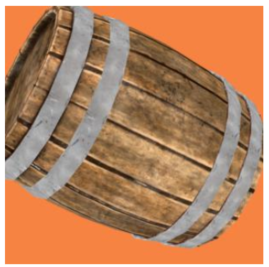
\includegraphics[width=0.4\linewidth]{./graphics/athalye_barrel.png}
}~ % Use a tilde to add spacing for sub-figures that are displayed next to one another horizontally.
\subfloat[Model used by this project.]{
	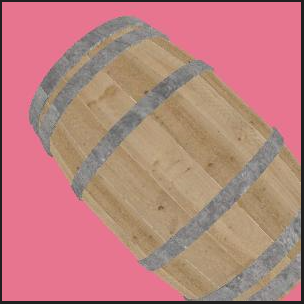
\includegraphics[width=0.4\linewidth]{./graphics/my_barrel.png}
}\\ % New line before caption.

\caption[Comparison of the camera distances used in Athalye \textit{et al.} versus this project.]{A comparison of an image of the barrel model used in Athalye \textit{et al.} versus an image of the barrel model used by this project.}
\label{fig:barrel_comparison}
\end{figure}

After creating the 50 adversarial textures, the same renderer used during the EOT optimisation process is used to create the evaluation images. For each adversarial texture, 100 images of the rendered object with that texture are created. For each image with the adversarial texture, an image of the object in the same pose and with the same background colour, but with the normal texture, is rendered. You can see an example of this in figure \ref{fig:evaluation_images_comparison}. This is done to observe the effect of using the adversarial texture rather than the original one, as all other factors are the same in the two images.

\begin{figure}[H]
\centering
\subfloat[Adversarial image.]{
	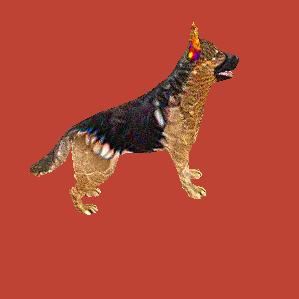
\includegraphics[width=0.485\linewidth]{./graphics/adv_dog_image.jpg}
}~ % Use a tilde to add spacing for sub-figures that are displayed next to one another horizontally.
\subfloat[Normal image.]{
	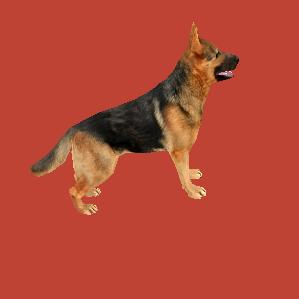
\includegraphics[width=0.485\linewidth]{./graphics/std_dog_image.jpg}
}\\ % New line before caption.

\caption[Comparison between equivalent adversarial and normal images for evaluation.]{Comparison between an evaluation image of the dog model with the adversarial texture versus its normal counterpart. The adversarial texture is for the "black grouse" target label.}
\label{fig:evaluation_images_comparison}
\end{figure}

\subsection{Experiment Results}
    \label{subsec:eot_experiment_results}

On the 5000 images with normal textures, the average classification accuracy was 60.28\%, while only 0.08\% of them were classified as the adversarial target label. By comparison, the 20000 normal images in Athalye \textit{et al.} \cite{athalye} had an accuracy of 68.8\% and only 0.01\% were classified as the target label. These figures are similar, although my images had a significantly lower classification accuracy. This is caused by the classification accuracies for normal images of the taxi and camaro models being only 15 and 10.8, as you can see in table \ref{table:model_labels_accuracy}. Without these two models, the average accuracy would be 72.125\%. 

But on the adversarial images, the average classification accuracy was just 0.86\%, very close to the EOT paper's result of 1.1\% \cite{athalye}. Meanwhile, the average TFR was 80.08\%, slightly under the TFR of 83.4\% seen in the EOT paper.  The mean TFR and the target labels for each individual model can be seen in table\ref{table:eot_results}. The slightly worse performance may be caused by a multitude of factors. Even though the dataset described in section \ref{sec:dataset} is designed to mimic the one used in \cite{athalye}, it is not identical. Furthermore, different values for the $\lambda$ penalty constant, learning rate, and the number of optimisation steps were used compared to \cite{athalye}, as the authors did not specify what values they used. 

The fact that the adversarial textures brought down the classification accuracy from 60.28\% to 0.86\%, and increased the TFR from 0.08\% to 80.08\%, demonstrates that this implementation of EOT \footnote{https://github.com/Alexandru-Dascalu/adversarial-3d} is highly effective at creating robust adversarial attacks for 3D rendered objects. Moreover, the results are very similar to those in \cite{athalye}, demonstrating that it is an accurate re-creation of the implementation used by the authors of that paper.

In figure \ref{fig:eot_histogram} you can see a histogram of the TFR for each of the 50 adversarial textures. You can see that 27 out of 50 adversarial textures had a mean TFR of over 90\%. Meanwhile, just 2 adversarial textures are failures, with a mean TFR under 20\%. This demonstrates that the vast majority of adversarial textures for 3D objects are highly successful.

\begin{figure}[ht]
    \centering
    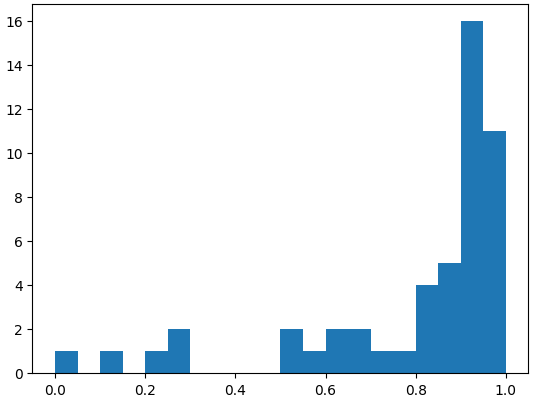
\includegraphics[width=0.7\textwidth]{graphics/eot_histogram.PNG}
    \caption{Histogram of TFR of the 50 adversarial examples.}
    \label{fig:eot_histogram}
\end{figure}

It took 82 hours to create the 50 adversarial textures on an RTX 3070 with 8GB of VRAM. That GPU can do around 2900 EOT optimisation steps in an hour, and therefore the creation of a single adversarial texture can take up to around 3.4 hours.

All 50 adversarial textures created by and used in this experiment can be seen in appendix \ref{app:adversarial_textures}.

\begin{table}
\caption{Results of the EOT experiment on rendered 3D objects.}
\label{table:eot_results}
\begin{tabular}{|p{2.6cm} | p{6.5cm} | p{2cm}| p{2cm}|} 
 \hline
 Model Name & Target Labels & Mean TFR (\%) & Mean number of iterations \\
 \hline
 barrel & file cabinet, hourglass, hautboy, purse, typewriter keyboard & 95.59 & 1428.4 \\ 
 \hline
 baseball & Australian terrier, dingo, indian elephant, radiator, warplane & 80.6 & 6349.2 \\
 \hline
 camaro & kite, mongoose, indri, trombone, red-breasted merganser & 93.39 & 2585.8 \\
 \hline
 clownfish & swimming cap, grand piano, shopping basket, wall clock, bridegroom & 48.2 & 10000 \\
 \hline
 german\_shepherd & bald eagle, barrel, bikini, black grouse, hornbill & 85.6 & 5243 \\
 \hline
 orange & whippet, goblet, lighter, missile, plate & 97.4 & 1163.2 \\
 \hline
 purse & pit bull terrier, chickadee, dhole, weevil, sandbar & 42.8 & 9090.6 \\
 \hline
 sea\_turtle & Australian terrier, leopard, mantis, cradle, plunger & 80.39 & 5123 \\
 \hline
 taxi & groenendael, marmot, acoustic guitar, cradle, radiator grille & 87.8 & 4229.6 \\
 \hline
 teddy & soft-coated wheaten terrier, leatherback turtle, pool table, hot pot, pineapple & 89 & 2782.8 \\
 \hline
\end{tabular}
\end{table}

\newpage
\subsection{Discussion}

\subsubsection{Classification accuracy on normal images}

The very low InceptionV3 classification accuracies for normal texture images of the taxi and camaro models of 15 and 10.8 per cent, respectively, might be caused by the fact that the objects are rendered with completely random rotations on the X, Y and Z axes. Therefore, these cars are often seen from below or above. The images of taxis or sports cars in the Imagenet dataset are of cars as they appear on the street, and therefore seen from the side, front or back, not from above or underneath.

Then again, the classification accuracy on images with the normal texture does not seem to impact the performance of EOT. The adversarial textures for taxi and camaro models had a mean TFR of 87.8\% and 93.39\%, respectively.

\subsubsection{EOT performance depending on the model}

Out of the two adversarial textures with a mean TFR of under 20\%, one is the adversarial texture for the clownfish model and the grand piano target label, the other is the one for the purse model and the pit bull terrier label. Even without those two, the mean TFRs of the clownfish and purse adversarial textures are around only 50\%. The ability of EOT to create adversarial examples seems to be influenced by the perceptual difference between the model and the target label. A clownfish has a vastly different shape and colour compared to a piano. In particular, the colour pattern of a clownfish is very distinct and different from a piano, and likely prevents the renders of the adversarial clownfish to be classified as a piano.

Similarly, the brown purse model has a very different colour from a pit bull terrier, resulting in a TFR of 1\% for that model. However, the purse adversarial texture for the Asian wild dog target label had a mean TFR of 62\%. The contrast may be explained by the fact that the wild dog is brown in colour, and thus already perceptually closer to the brown purse.

Models with a simple shape, similar to a sphere, and/or a colour pattern dominated by one simple colour, seem to be a better "canvas" for EOT to apply adversarial noise on. The barrel and orange 3D models have a mean TFR of over 90\%, as you can see in table \ref{table:eot_results}. The camaro and taxi models mostly have a solid yellow colour and they have a mean TFR of over 85\%. On the other hand, models with more complicated shapes like the sea turtle and the german shepherd have a lower mean TFR. 

A simple colour ensures that EOT can gradually develop adversarial patterns more easily, while a simpler shape means that the model looks similar regardless of the angle it is viewed from, which makes the gradient fluctuate less despite the random poses the model is rendered in.

\subsubsection{Number of iterations}

As subsection \ref{subsec:eot_experiment_design} mentioned, the algorithm stopped when the average loss of the past 400 steps was below 0.5 or ran for at most 10000 steps. Table \ref{table:eot_results} displays the average number of iterations it took to create the five adversarial examples for each model. It is likely that the threshold for stopping the algorithm could have been set to 0.8 instead of 0.5 to reduce runtime while obtaining similar TFRs.

Unsurprisingly, the models with the lowest mean TFR, the clownfish and the purse, also took the longest to create. Meanwhile, the models with a simpler texture and colour were easier to optimise. For example, it took EOT on average just 1163.2 iterations to run for the orange model. 

The number of necessary optimisation steps is influenced by the somewhat random nature of the gradient, caused by the fact that each rendered image in the batch is random. This perceptual randomness is smaller for models with a simple shape, as they look similar regardless of the angle they are seen from. As you can see in figure \ref{fig:eot_orange_loss_history}, the loss value fluctuates very little for the orange model, leading to much faster convergence. At the other extreme, the loss value for the clownfish model and shopping basket target label fluctuates wildly, sometimes from a value of 1 to 3 or even 4, as you can see in figure \ref{fig:eot_clownfish_loss_history}. The "Main loss" in these loss history plots refers to the value of the first term in equation \ref{eq:eot} in subsection \ref{subsubsec:eot_technique}, while "L2 Loss" refers to the penalty constraining the size of the adversarial perturbation in that equation. "Total Loss" refers to the sum of these two terms.

\begin{figure}[ht]
    \centering
    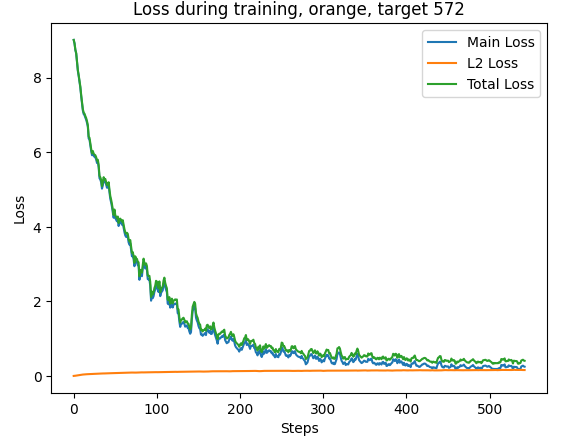
\includegraphics[width=0.7\textwidth]{graphics/eot_orange_loss_history.PNG}
    \caption[Optimisation history for the orange model and target label goblet.]{Optimisation history for the orange model and target label goblet. L2 loss refers to the penalty term in equation \ref{eq:eot}, main loss refers to the first term. Its evaluation TFR is 100\%.}
    \label{fig:eot_orange_loss_history}
\end{figure}

\begin{figure}[ht]
    \centering
    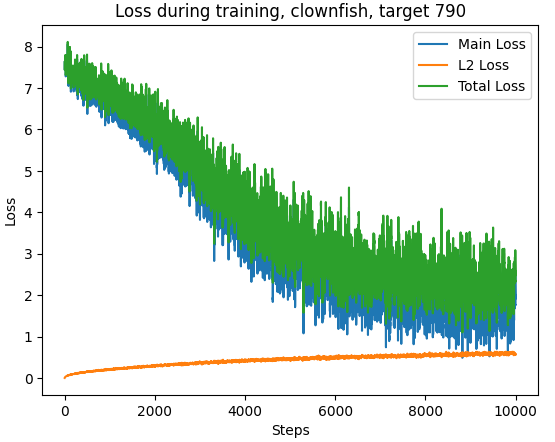
\includegraphics[width=0.7\textwidth]{graphics/eot_clownfish_loss_history.PNG}
    \caption[Optimisation history for the clownfish model and target label shopping basket.]{Optimisation history for the clownfish model and target label shopping basket. Its TFR is 71\%.}
    \label{fig:eot_clownfish_loss_history}
\end{figure}

Another interesting observation is that the longer the EOT algorithm has to run, the more noisy the created adversarial textures will be. You can see this in the textures in figures  \ref{fig:clownfish_noisy_texture} and \ref{fig:dog_noisy_texture}, both of which took the maximum number of 10000 steps to create.

\begin{figure}[H]
    \centering
    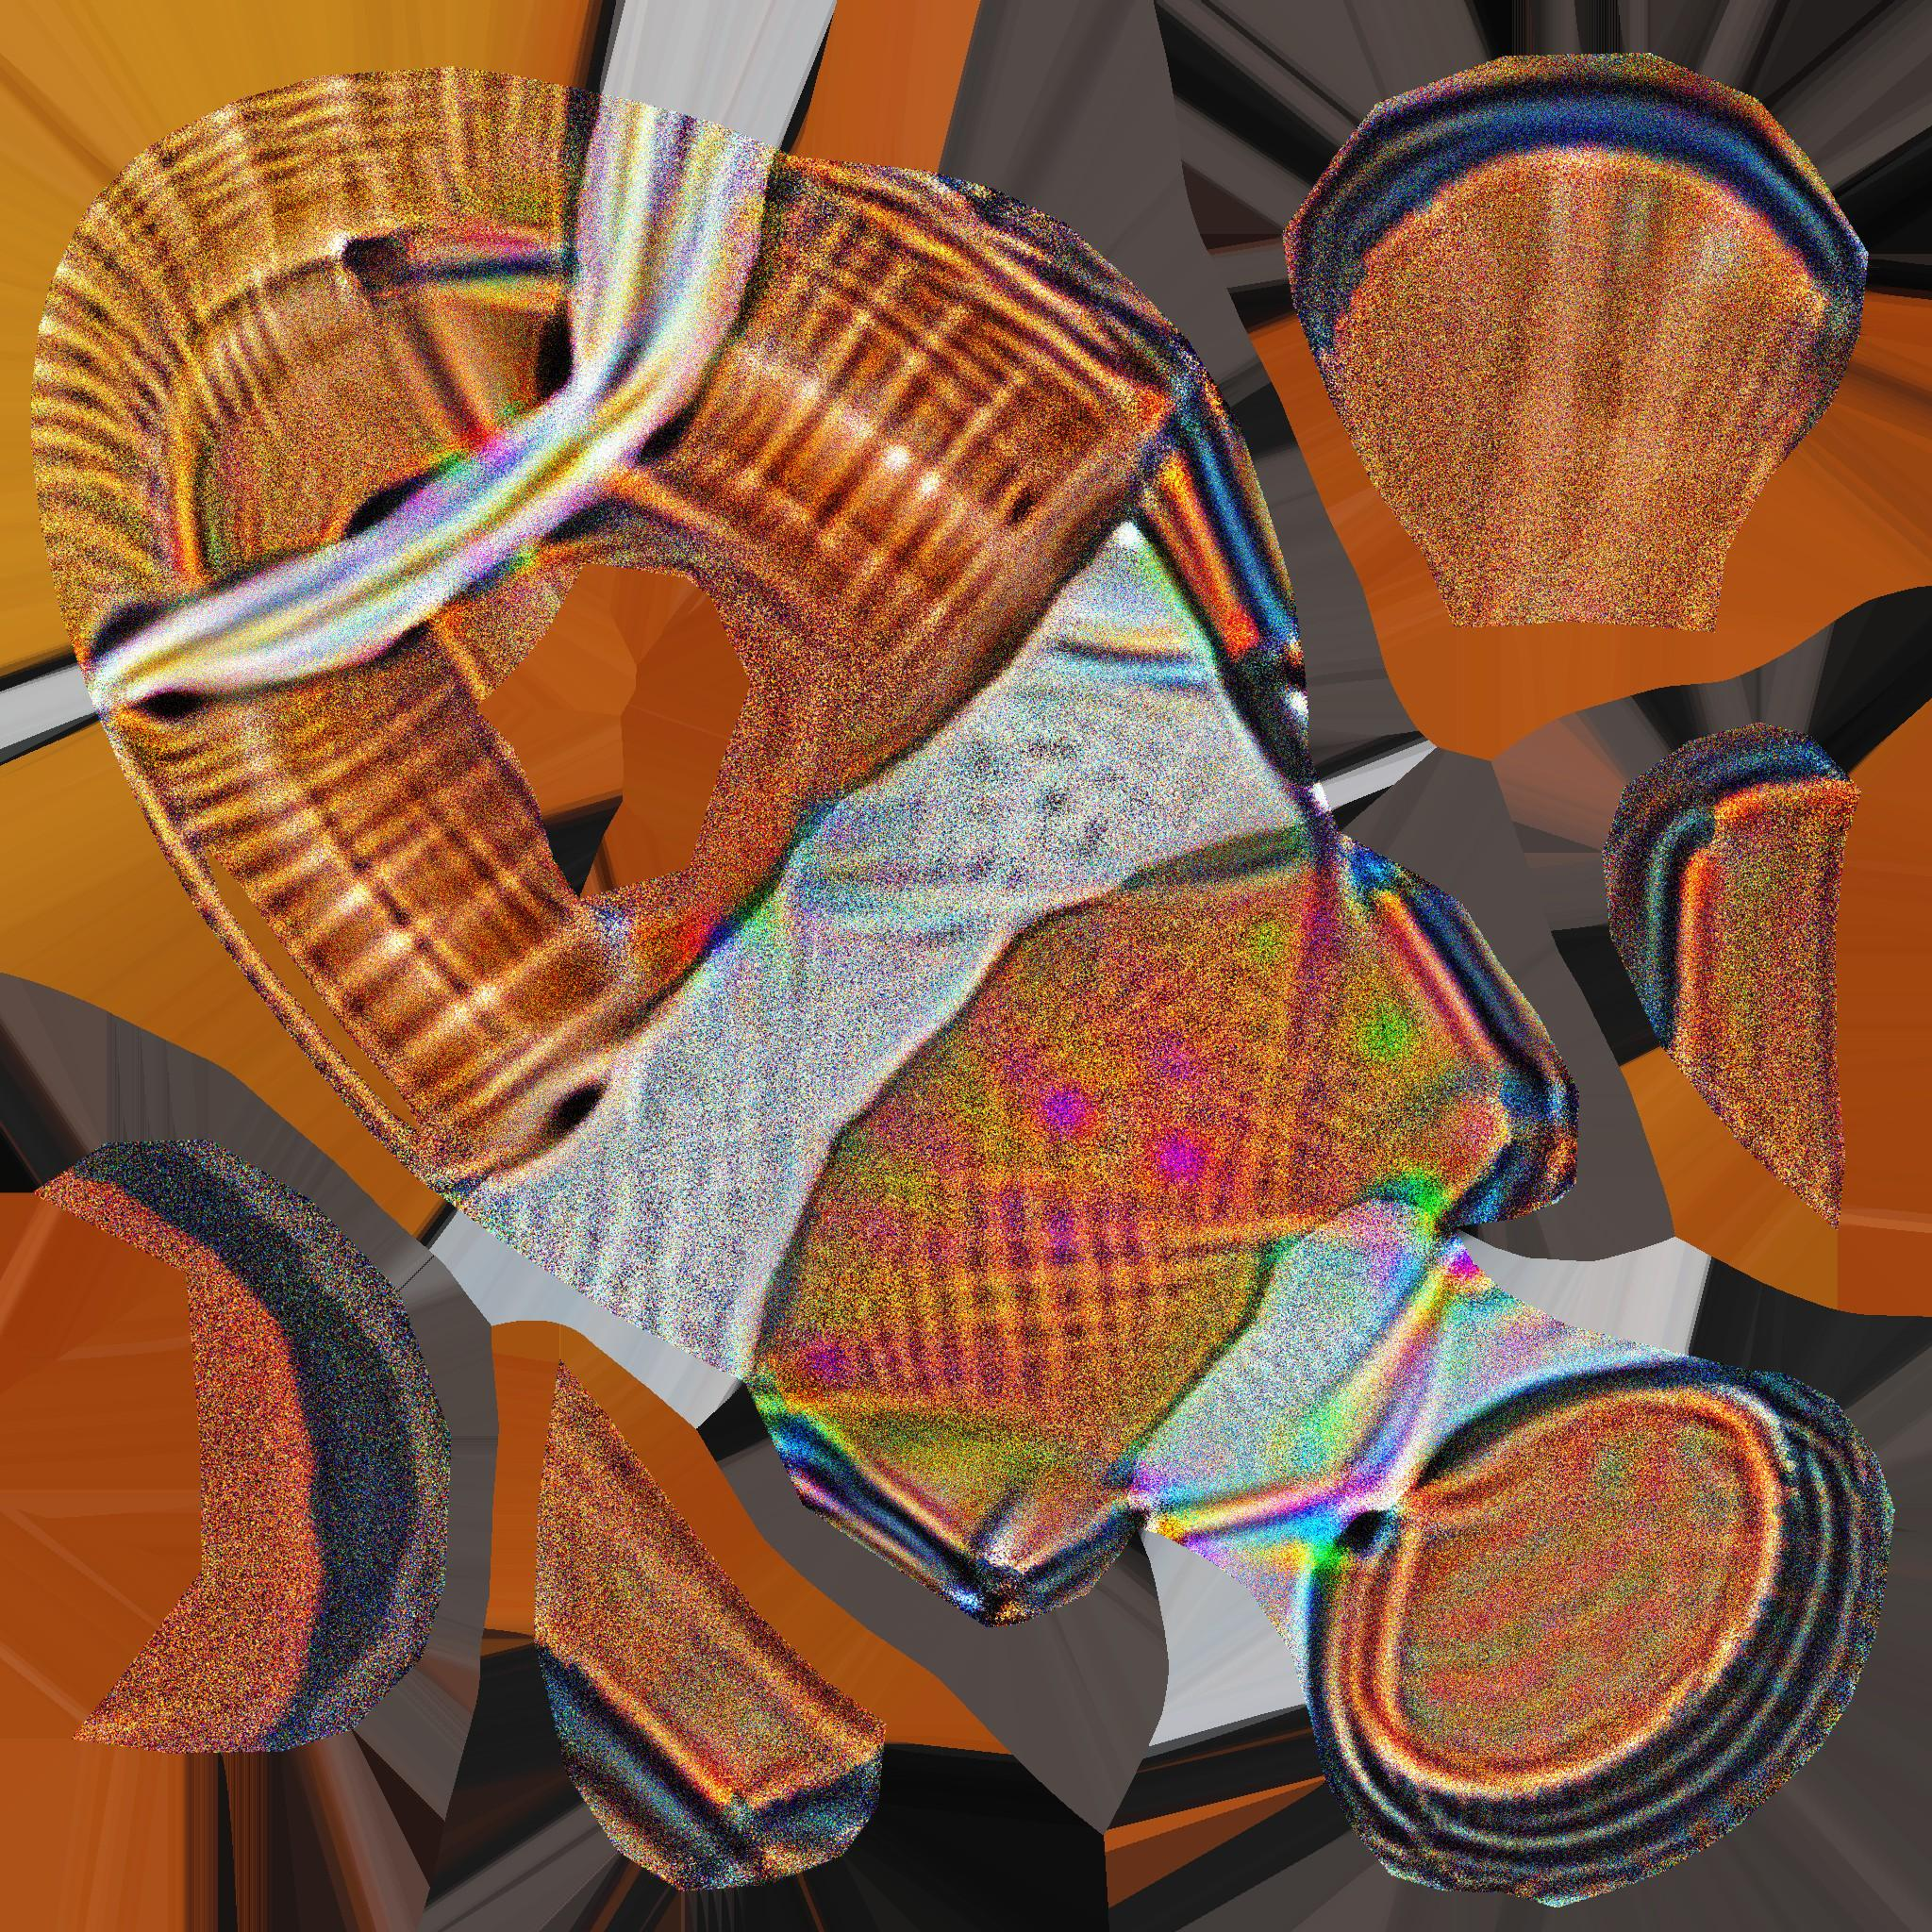
\includegraphics[width=0.6\textwidth]{graphics/clownfish_790_adv_9999.jpg}
    \caption[Adversarial texture for the clownfish model and target label shopping basket.]{Adversarial texture for the clownfish model and target label shopping basket. Its TFR is 71\%.}
    \label{fig:clownfish_noisy_texture}
\end{figure}

\begin{figure}[H]
    \centering
    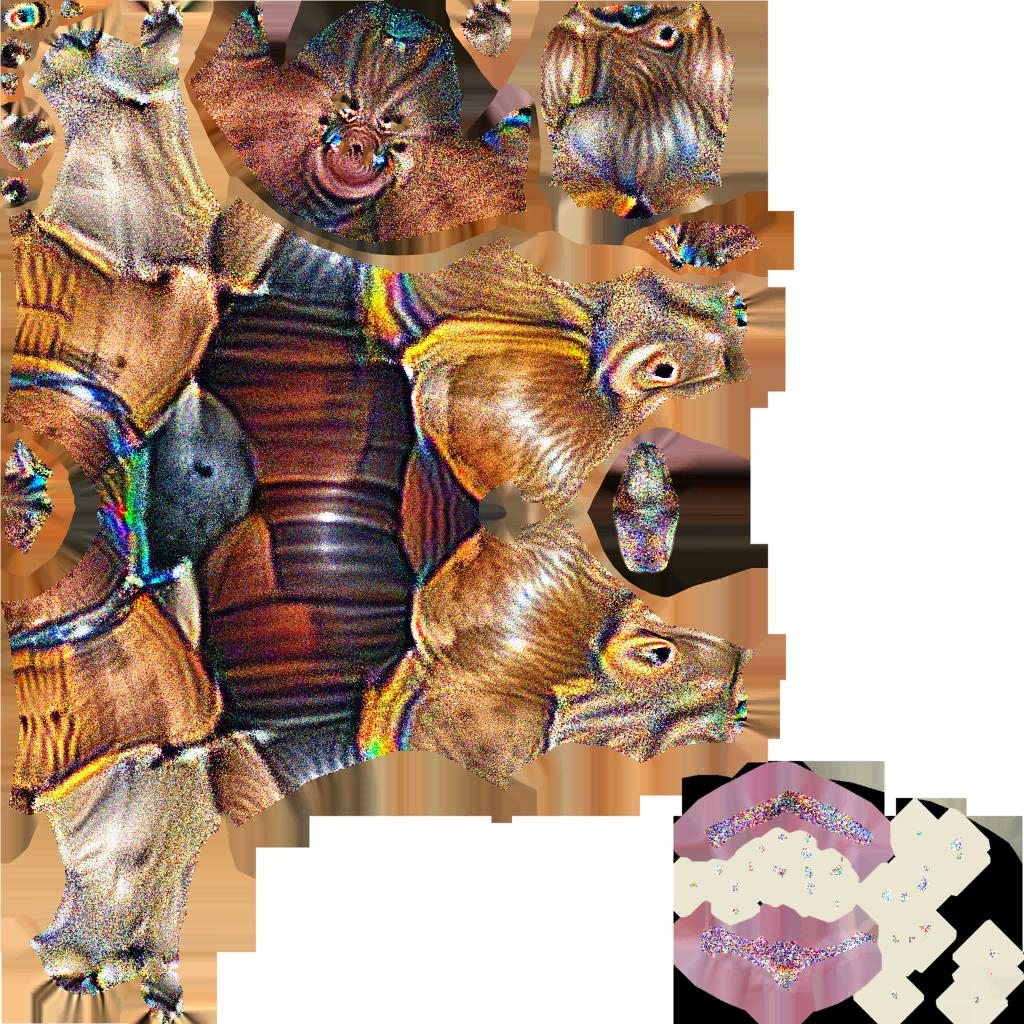
\includegraphics[width=0.6\textwidth]{graphics/german_shepherd_427_adv_9999.jpg}
    \caption[Adversarial texture for the german shepherd model and target label barrel.]{Adversarial texture for the german shepherd model and target label barrel. Its TFR is 76\%.}
    \label{fig:dog_noisy_texture}
\end{figure}

\subsubsection{Reusing renders between optimisation steps}

Some ad-hoc experiments done with the barrel model, before the experiment in subsection \ref{subsec:eot_experiment_design}, show that re-using 80\% of renders versus re-using none has little effect in terms of the TFR of adversarial texture. However, it greatly speeds up the EOT algorithm, as it can do the same number of optimisation steps in less than half the time. It shows that one of the most computationally intensive parts of EOT is the computation of UV maps and using the latter to render 2D images of the objects, as Athalye \textit{et al.} \cite{athalye} also suggested.

\subsubsection{Semantic adversarial perturbations}

A key characteristic of the adversarial noise made for textures of 3D objects by EOT is that they show semantically meaningful patterns related to the target class. A different experiment from the one described in subsection \ref{subsec:eot_experiment_design}, on the crocodile 3D model and target label compass, resulted in the texture in figure \ref{fig:crocodile_compass}. EOT added noise on the belly and back of the crocodile with an oval or circular shape, the same shape a compass has. Similarly, you can see in figure \ref{fig:running_shoe_strawberry} that EOT added green spots, reminiscent of the green seeds on a strawberry, for an adversarial texture of the running shoe model for the strawberry target label.

\begin{figure}[H]
    \centering
    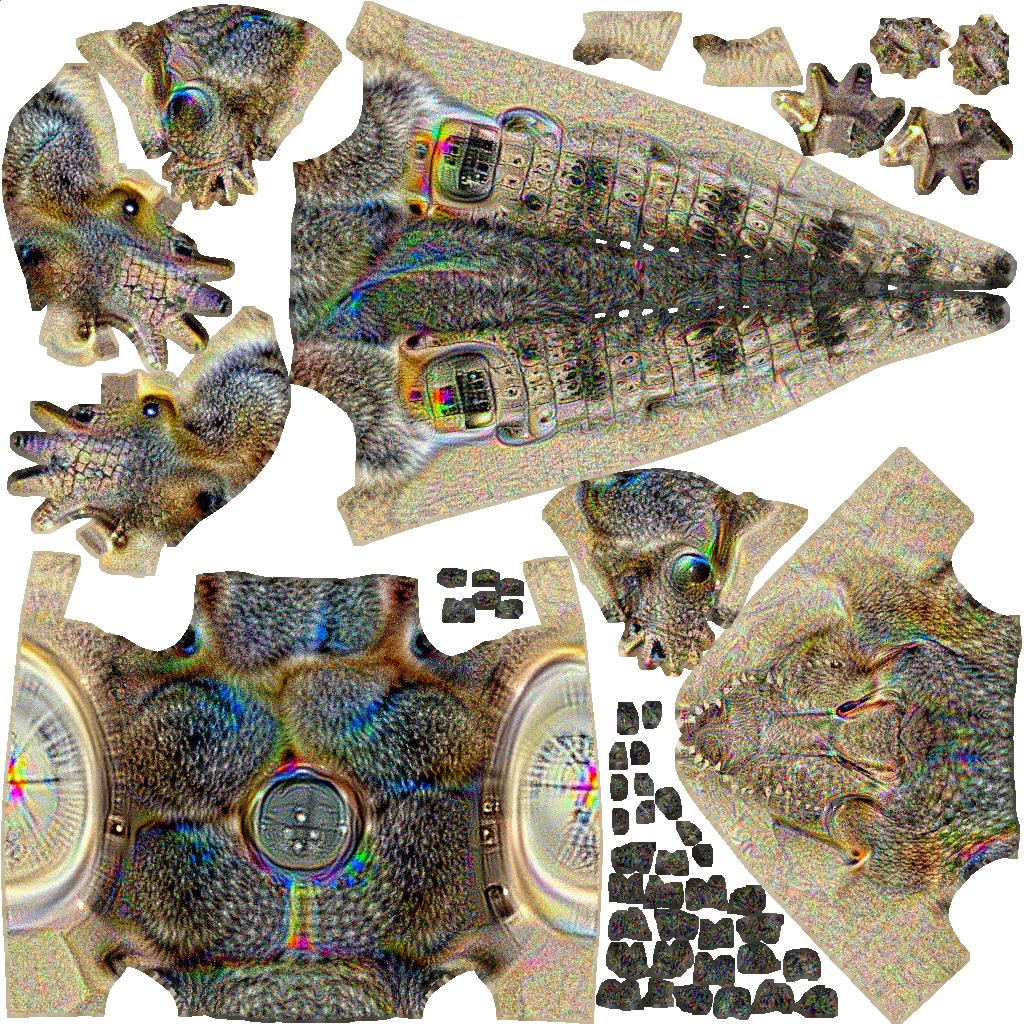
\includegraphics[width=0.55\textwidth]{graphics/crocodile compass.jpg}
    \caption[Adversarial texture for the crocodile model and target label compass.]{Adversarial texture for the crocodile model and target label compass. It has a TFR of 60\%.}
    \label{fig:crocodile_compass}
\end{figure}

\begin{figure}[H]
    \centering
    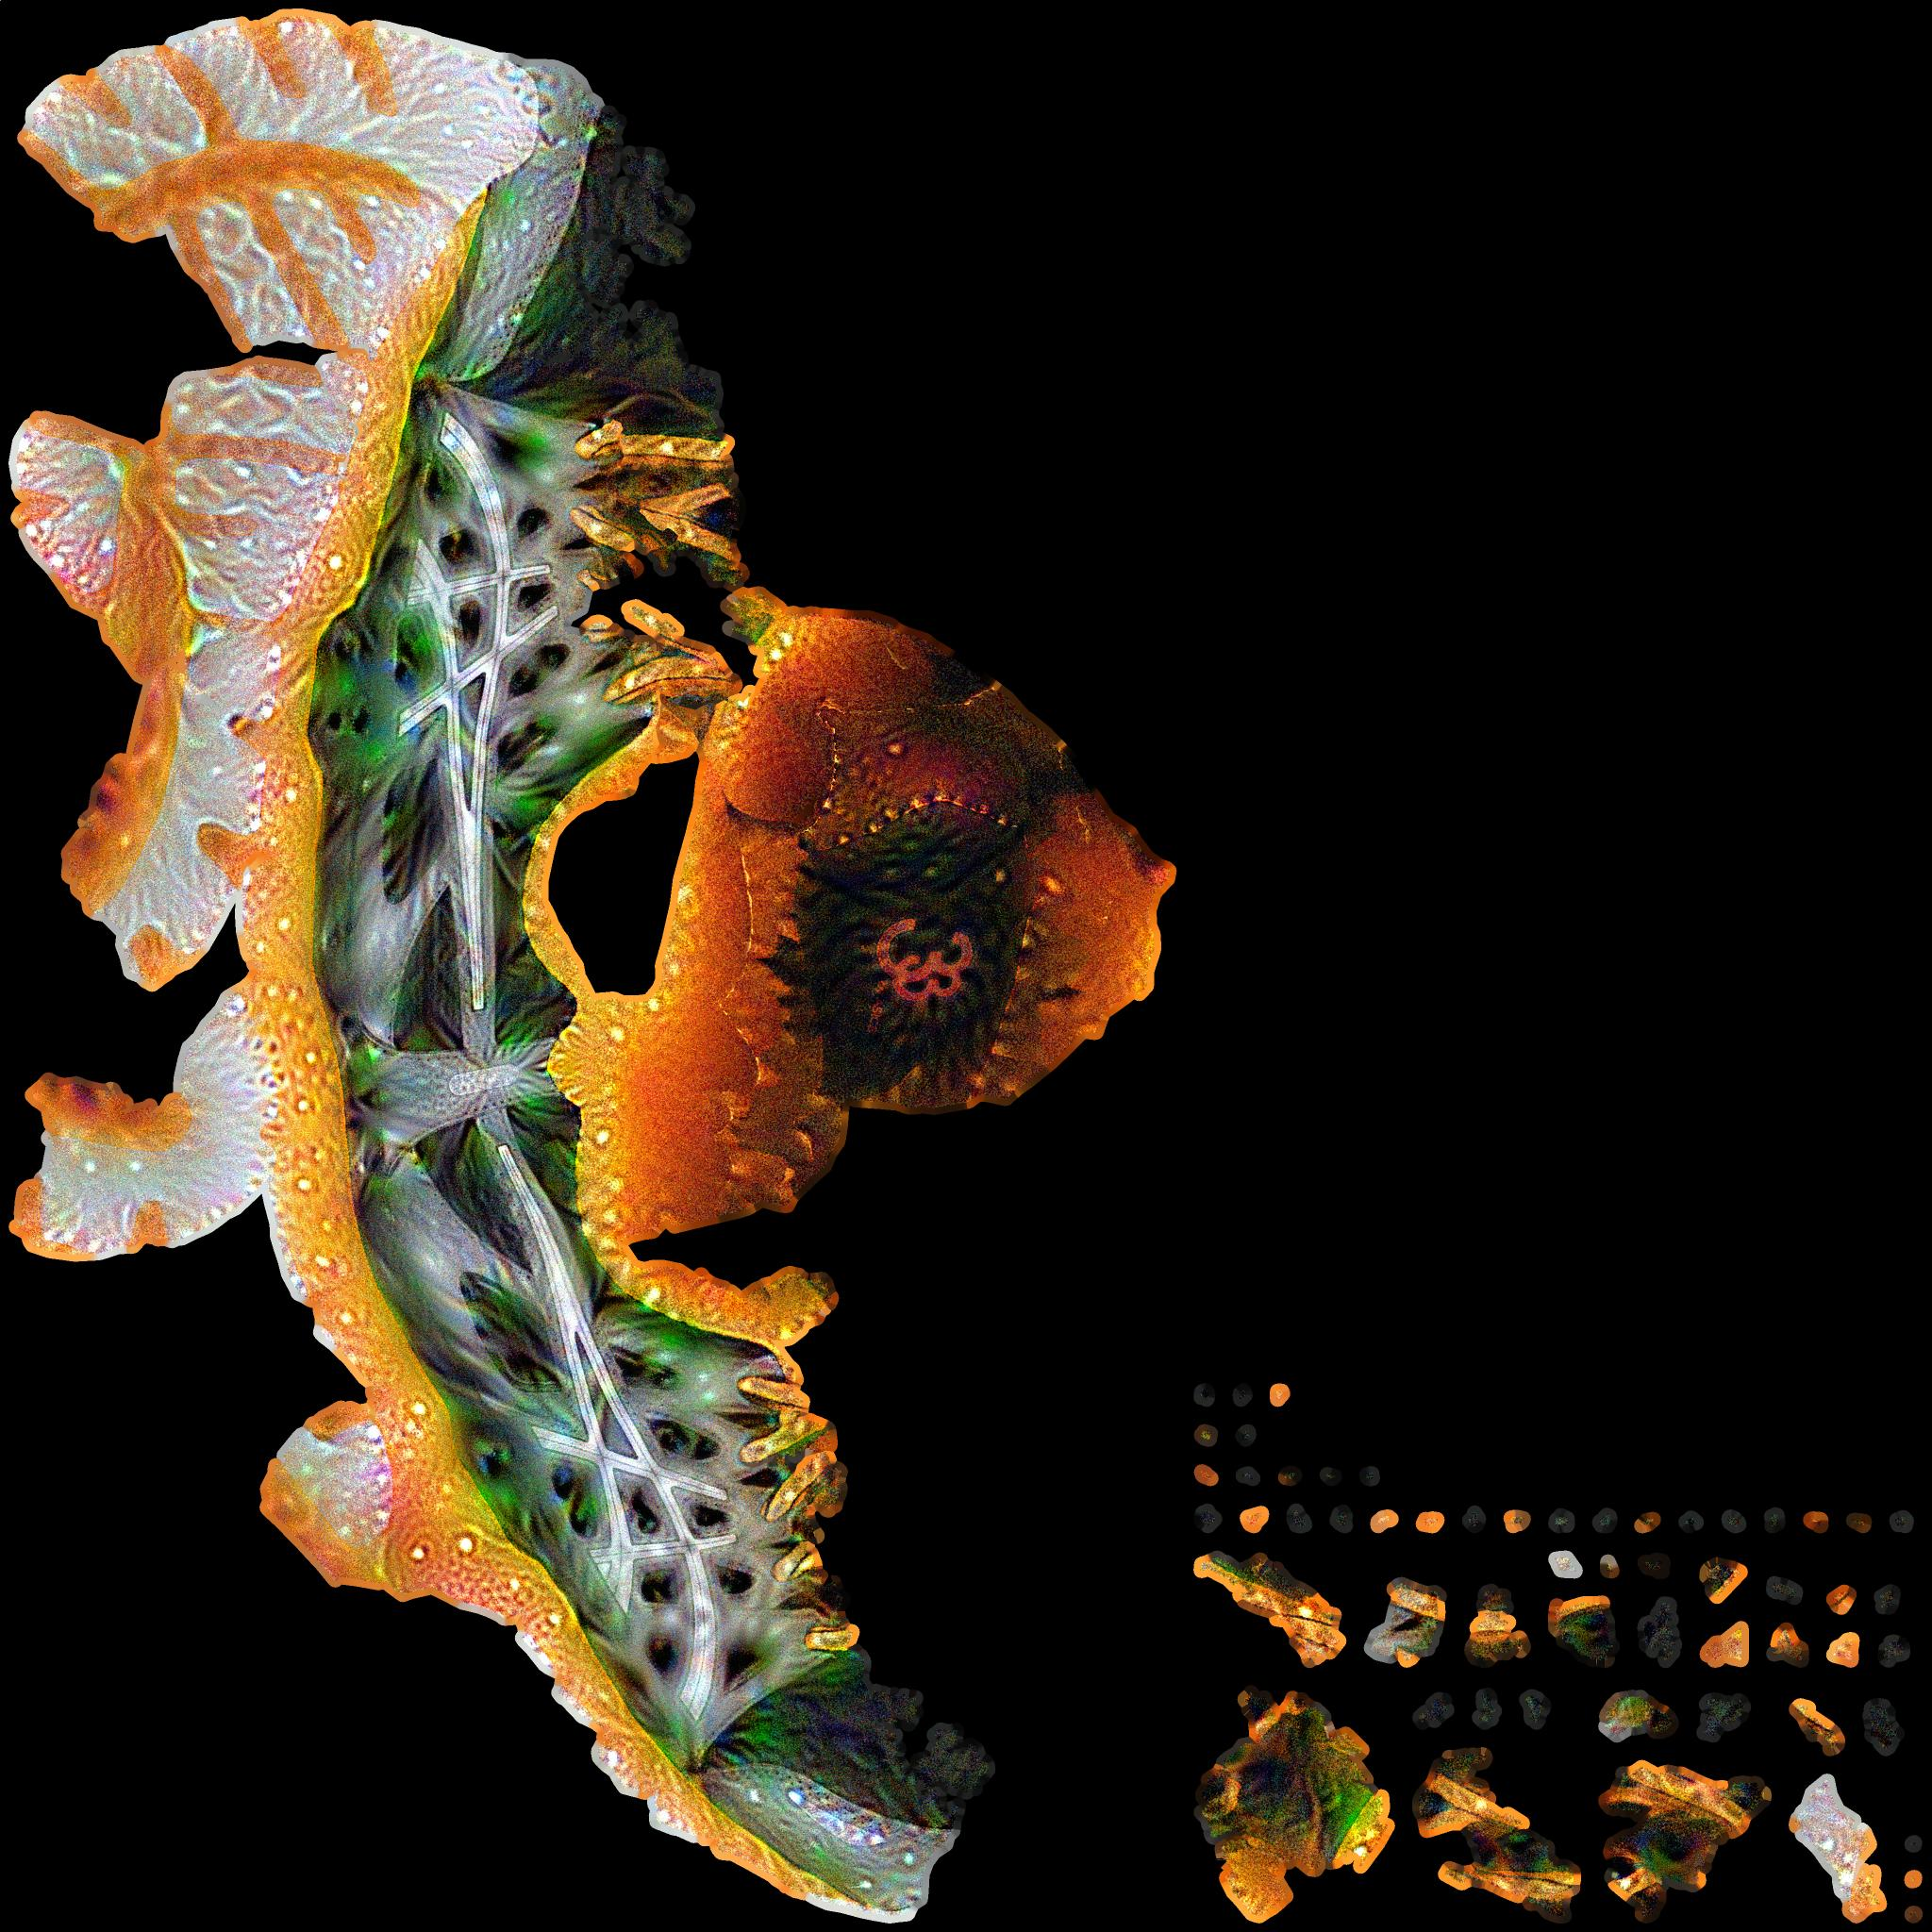
\includegraphics[width=0.55\textwidth]{graphics/running shoe strawberry.jpg}
    \caption[Adversarial texture for the running shoe model and target label strawberry.]{Adversarial texture for the running shoe model and target label strawberry. It has a TFR of over 80\%.}
    \label{fig:running_shoe_strawberry}
\end{figure}

Another example is in figure \ref{fig:running_shoe_rifle}, where the adversarial texture for the running shoe and target label rifle exhibits metallic patterns in the shape of a gun barrel. Given that these three adversarial textures have a significant TFR, they highlight features that the InceptionV3 victim model learned for recognising a compass, strawberry and rifle, respectively. Therefore, EOT can be used to study the explainability of a neural network, as it highlights class features that make the neural network classify a completely different object as that class.

\begin{figure}[H]
    \centering
    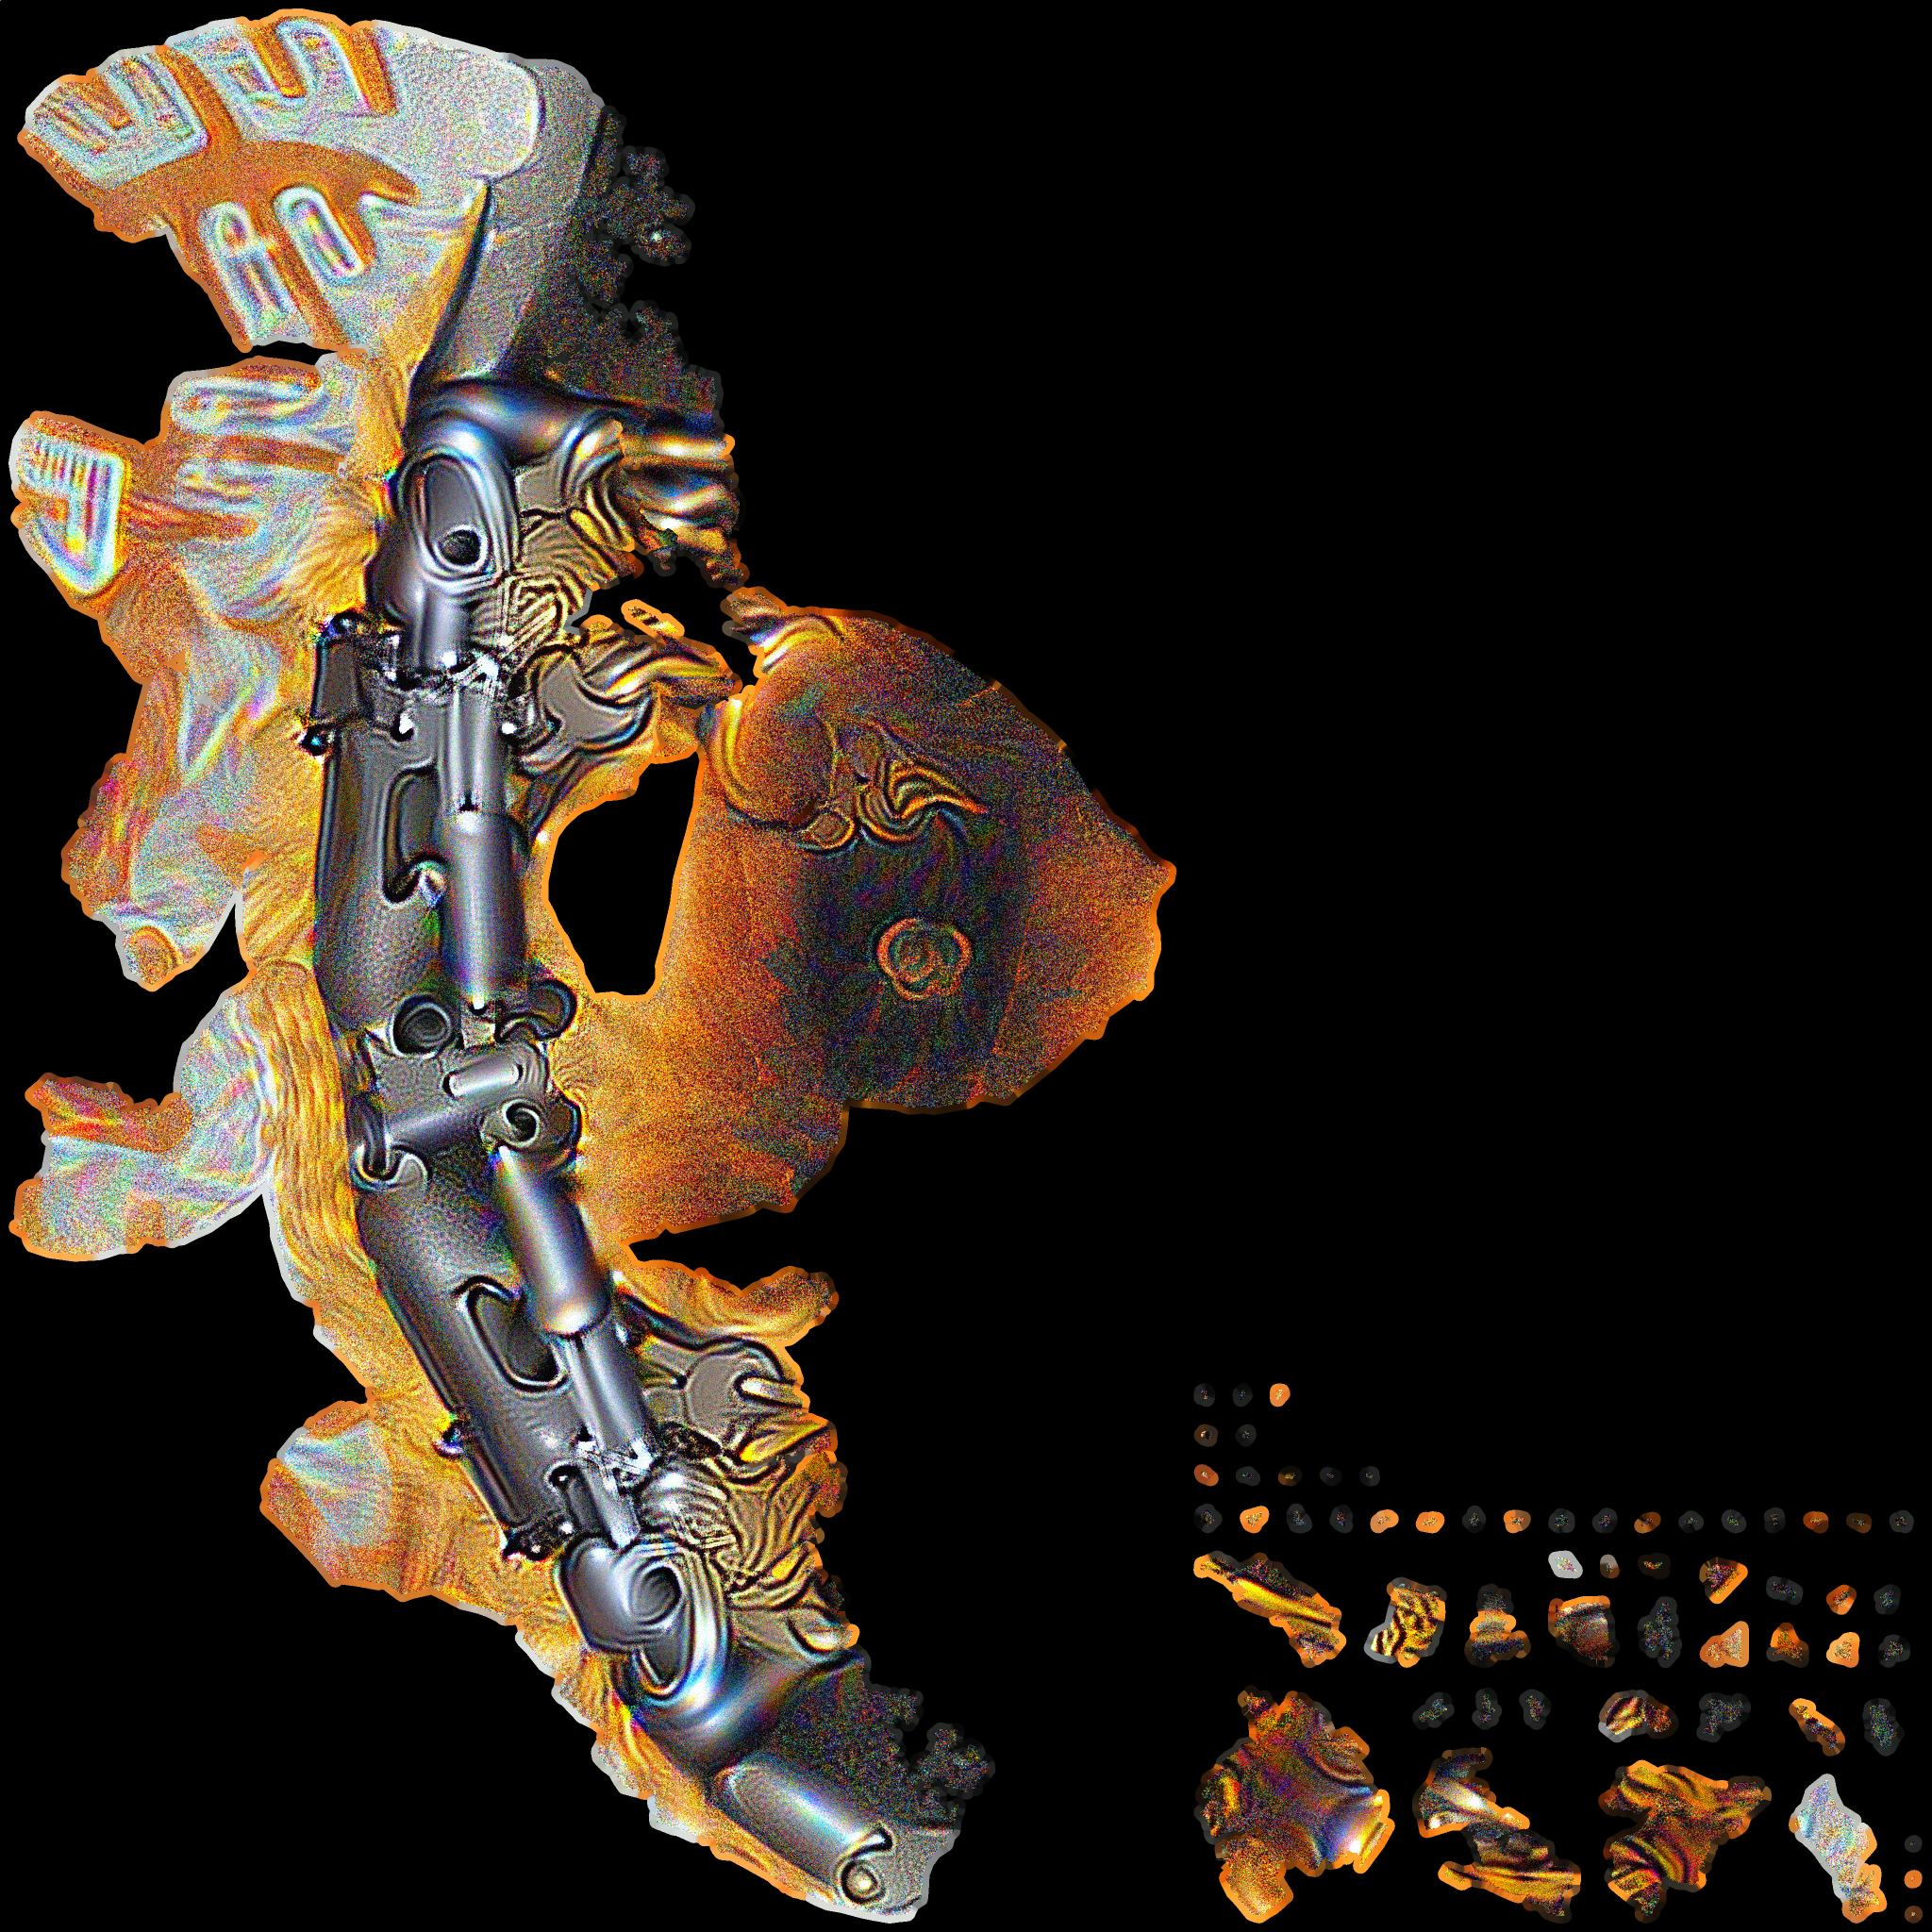
\includegraphics[width=0.55\textwidth]{graphics/running shoe rifle.jpg}
    \caption[Adversarial texture for the running shoe model and target label rifle.]{Adversarial texture for the running shoe model and target label rifle. It has a TFR of 45-50\%.}
    \label{fig:running_shoe_rifle}
\end{figure}

\section{G-EOT}

\subsection{Experiment Design}
    \label{subsec:g_eot_experiment_design}

The purpose of this experiment is to see if G-EOT is able to learn to create adversarial noise for textures. The model is evaluated by training it using the process described in subsection \ref{subsec:training} to attack Tensorflow Keras' pre-trained Xception neural network classifier \cite{xception}. This target was chosen because the simulator's architecture is inspired by Xception, and therefore training the simulator to distil that model should be easier compared to a different architecture.

Firstly, the simulator is warmed-up for 2000 training steps. Following that, the G-EOT model is trained for 40000 steps, where each one consists of one simulator training step and one generator training step. This number was chosen because training the model made by Zheng \textit{et al.} \cite{zheng_black_box_GAN} took around 30000 steps to achieve the results seen in their paper, and G-EOT has a harder generation task. Every 500 training steps, the generator is evaluated on 200 batches of new data samples that the generator has not seen before.

The model is trained on the dataset of 15 3D models presented in section \ref{sec:dataset}. At each training step, the batch is made up of randomly picked models out of this dataset. For each model in the batch, random parameters are sampled for translation, rotation and distance from the camera, and a UV map is computed based on those. Moreover, a random target label is sampled from a uniform distribution. It can be any of the 1000 Imagenet labels, except the correct labels for that model. Therefore, each element in the batch is a randomly picked model, with a UV map for a random pose and a random target label. In this experiment, the batch size is 5, as that is the maximum that will fit in 8 GB of VRAM. An Nvidia RTX 3070 graphics card is used for this experiment.

The bounds for the uniform distributions used for sampling the camera distance, X/Y translation, additive and multiplicative lighting, and the standard deviation of the gaussian noise, are the same as those used for the EOT experiment in subsection \ref{subsec:eot_experiment_design}. This experiment does not scale the texture before rendering in order to simulate 3D printer errors, as the adversarial 3D models will not be physically printed.

The number of experts in the decoder is 50, as having one expert for each of the 1000 Imagenet labels would be too much, and different combinations of expert outputs can be used for each target label. The simulator uses an Adam optimiser with an exponentially decaying learning rate. The initial learning rate is 0.001, with a decay rate of 0.98, and it decays after every 300 steps. The generator uses a constant learning rate of 0.004. The reason is that the random renders can lead to strong fluctuations in the loss function value, as you have seen in subsection \ref{subsec:eot_experiment_results}, and a large constant learning rate mitigated that and improved performance for the EOT experiment in \ref{subsec:eot_experiment_results}. The gradients of the generator loss function are clipped to a range between -1 and 1, as Zheng \textit{et al.} \cite{zheng_black_box_GAN} also did.

The noise produced by the G-EOT generator has individual values for each pixel between -25 and 25, to be applied to images with pixel values between 0 and 255. The reason behind this limitation is that when training starts, the randomly initialised weights are very small, and therefore the values of the generated noise tend toward 0. When they are scaled to values between -1 and 1, these values are mostly -1. When added to a texture with pixel values between 0 and 1, this resulted in a completely black image. The simulator would not provide a useful gradient to the generator when given a black image, and therefore I introduced this limitation to avoid this. Further work should look into initialisation techniques to avoid this issue.

The weight $\beta$ from equation \ref{eq:g-eot-l2-loss} on page \pageref{eq:g-eot-l2-loss} has a value of 0.001, chosen to relax the constraint on the size of the adversarial noise and make the learning task for the generator easier. Finally, the weight for L2 regularisation of the weights of the simulator and generator is $0.5 * 10^{-4}$, and the simulator and generator's weights are initialised with Orthogonal Initialisation, which was used in BigGAN \cite{big_gan}.

\subsection{Experiment Results}
    \label{subsec:g_eot_experiment_results}
    
You can see a history of the loss of the model during training in figure \ref{fig:g_eot_loss_history}. The orange plot denotes the value of the first term of equation \ref{eq:generator_loss} on page \pageref{eq:generator_loss}, which measures how close is the generator to fooling the simulator. The green plot denotes the value of the term seen in \ref{eq:g-eot-l2-loss} on page \pageref{eq:g-eot-l2-loss}, which constrains the size of the adversarial noise. The red line represents the average generator loss at each evaluation step, which is done once every 500 training steps, as mentioned in the previous subsection. Moreover, this test loss is calculated by using the victim model rather than the simulator, as fooling the victim model is the intended objective.
    
\begin{figure}[H]
    \centering
    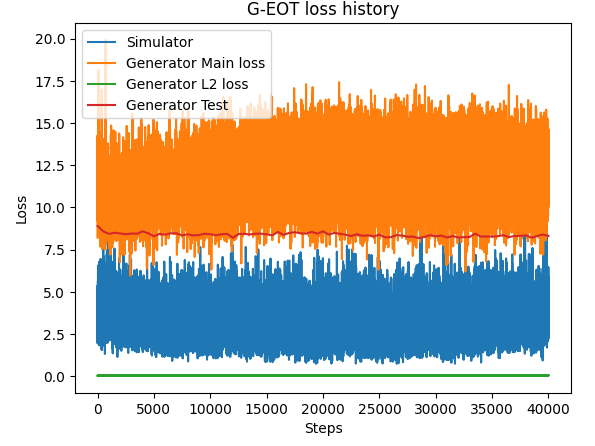
\includegraphics[width=1\textwidth]{graphics/g_eot_loss_exp1.PNG}
    \caption{Loss history during training for the G-EOT model.}
    \label{fig:g_eot_loss_history}
\end{figure}

The figure shows that the gradient for the generator fluctuates wildly between training steps. Moreover, despite a small decrease in the generator main loss and the generator test loss at the very beginning, they do not decrease further during training. Therefore, the generator failed to learn almost anything, having a TFR of almost 0\% for new random renders sampled during evaluation steps. Interestingly, the loss of the simulator also varies wildly between training steps and does not have a downward trend throughout training, despite its training task being a lot simpler. The loss of the simulator is a lot lower than the generator's, likely due to the simulator warm-up before training, at the end of which the simulator had an accuracy of 28.4\% on never before seen test samples.

The simulator has 9.75 million trainable parameters, almost half of the 22.8 million trainable parameters of Xception \cite{xception}. Given that distillation allows models to learn to imitate much larger models \cite{distillation}, and that during warmup the simulator's accuracy went from 0 to 28.4\%, the training technique of the simulator should not be a cause of the wild fluctuations of the simulator loss seen in figure \ref{fig:g_eot_loss_history}. Instead, the intuition is that the generator keeps changing its pattern of adversarial noise, and therefore the simulator has a high loss when trying to predict the same labels that the victim model predicts on the adversarial images.

The training task for the generator is significantly more difficult than that for the generator in Zheng \textit{et al.} \cite{zheng_black_box_GAN}. Its task is to learn to generate adversarial textures for 1000 target labels for each of the 15 3D models, such that the textures remain adversarial regardless of the random rendering of the model. You can see in figure \ref{fig:eot_clownfish_loss_history} in page \pageref{fig:eot_clownfish_loss_history} that using EOT to optimise just one texture for one target label can have large variations in the gradient between consecutive steps, and it takes thousands of optimisation steps with a large batch size to produce good results. A hypothesis for why the generator does not learn much is that the gradient changes too much between training steps, and therefore does not provide a useful training direction.

To test this hypothesis, I simplified the training task so that the generator only learns to create perturbations for 10 target labels. These are Imagenet labels 281 to 290, which represent 5 different cat breeds, puma, lynx, leopard, snow leopard and jaguar. These felines have specific fur colour patterns that should be easy to learn to generate and apply to textures. Consequently, the number of experts in the decoder was reduced from 50 to 10, and the smaller model allowed the batch size to be increased to 9. All other hyper-parameters are the same.

\begin{figure}[ht]
    \centering
    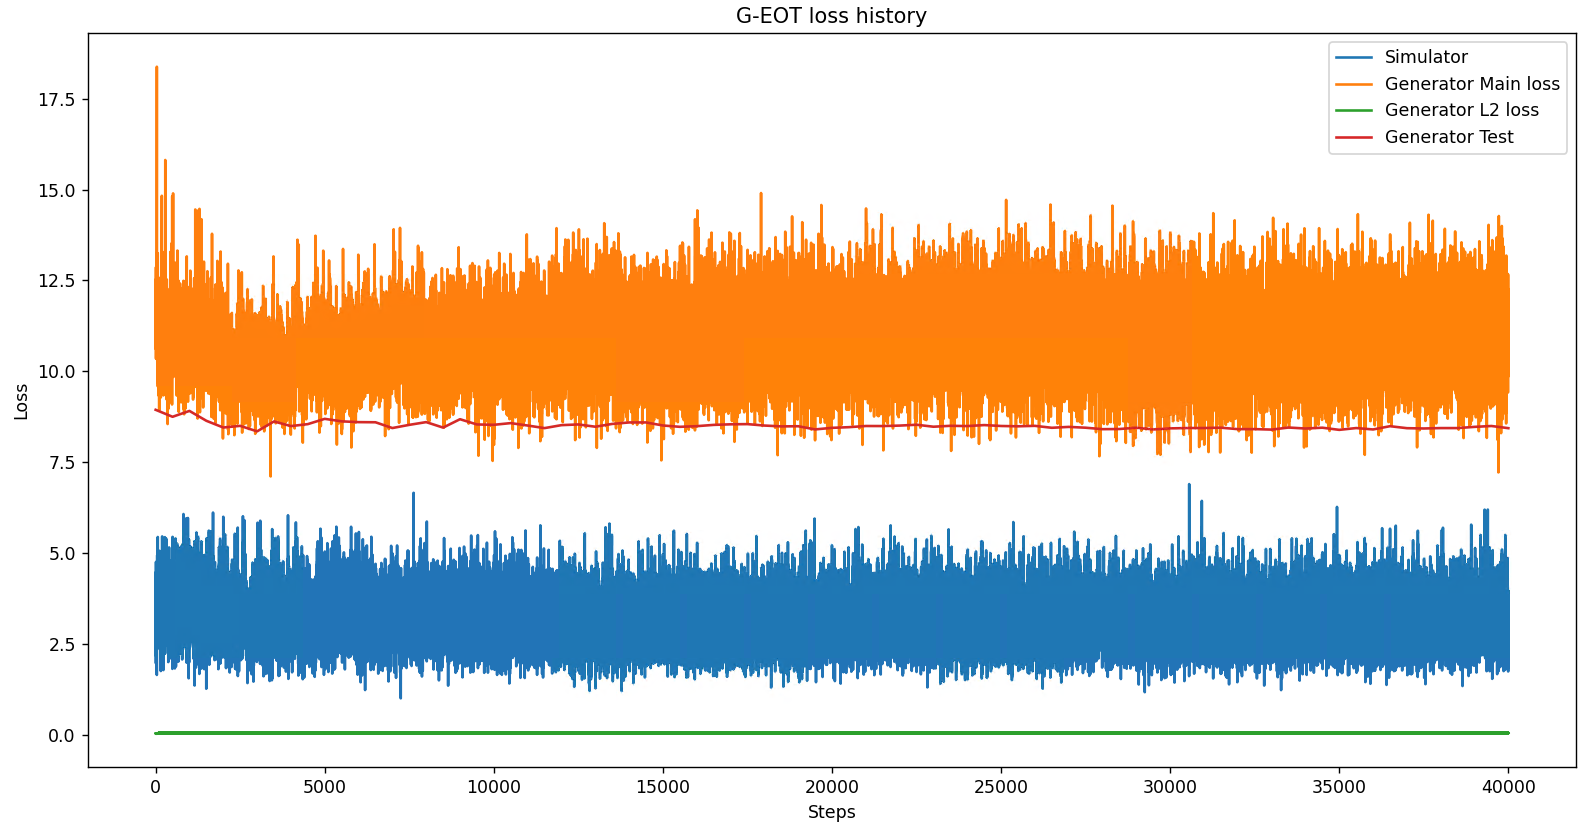
\includegraphics[width=1\textwidth]{graphics/g_eot_loss_exp2.PNG}
    \caption{Loss history during training for the G-EOT model for 10 target labels.}
    \label{fig:g_eot_loss_exp2}
\end{figure}

You can see the result in figure \ref{fig:g_eot_loss_exp2}. Unfortunately, the generator and simulator loss exhibit the same behaviours. While the generator's main loss and test loss decreased during the first 2000 steps, they made no improvements after. The value of the main term of the generator loss during training still has wild variations. However, while in figure \ref{fig:g_eot_loss_history} the generator main loss varies between 7.5 and 15, in figure \ref{fig:g_eot_loss_exp2} it varies roughly between 8.5 and 13.5. This shows that decreasing the number of target labels made the task easier, but it was not enough.
    
\subsection{Discussion}

As mentioned in the previous subsection, the intuition is that the generator failed to learn much due to the random image renders not giving a stable enough gradient. This issue was seen in the EOT experiment in subsection \ref{subsec:eot_experiment_results} for just 1 texture and one target label, yet the Adam optimiser could overcome that. However, trying to learn a distribution of adversarial noise for 15 textures and 1000 or 10 target models was too much. Therefore, more background reading needs to be done on initialisation, regularisation, training techniques, etc. for generative models that would mitigate the issue of the random gradient.

With 50 experts in the decoder, the generator has 36.1 million trainable parameters, and with 10 experts it has 20.5 million trainable parameters. Brock \textit{et al.} \cite{big_gan} used models with between 71.3 and 173.5 million parameters to generate images with sizes between 128x128 and 512x512. The G-EOT model may be able to learn better if it has a lot more parameters. However, such a large model would probably not be able to use a batch size larger than 1 with just 8 GB of VRAM. Therefore, a lot more computational resources might be needed to train a model such as G-EOT.

Moreover, even if a modified G-EOT would be able to complete its learning task, it might not be that useful for an attacker. In the experiment in subsection \ref{subsec:eot_experiment_results}, EOT took on average 1.64 hours to create an adversarial texture, with 3.3 hours being the maximum. A malicious agent would attack a neural network with a specific goal in mind, and therefore with a certain adversarial object and with a specific target label. They might be able to choose a 3D model of their choosing. For example, if they want to fool a facial recognition model in the real world, they may choose to add adversarial noise to a face mask, a pair of glasses, or something else worn by a person. The target label would be a different person, who has access to the room or space to which access is restricted by facial recognition. In another scenario, the attacker may want to trick a self-driving car into doing a particular action when seeing an adversarial road sign. In this case, the type of road sign to which adversarial noise is applied is not controlled by the attacker. But in both scenarios, the attacker only needs adversarial noise for one object and one target label, not for any of the 15 3D models and any arbitrary target label. And training G-EOT for 40000 steps took around 34.6 hours, more than 10 times more than it takes to use EOT to create an adversarial texture for a 3D model. Therefore, EOT would be more convenient for an attacker and is suitable for their task. Although EOT, as seen in Athalye \textit{et al.} \cite{athalye}, is a white-box attack method, it can become a black-box method by using distillation \cite{distillation} to train a simulator which behaves just like the victim model and then differentiate through the simulator to create the adversarial texture. Training the simulator should not take more than a couple of hours.

On the other hand, G-EOT could still be useful for adversarial training, which entails including adversarial examples in the training set of machine learning models so that they learn to classify them with the correct label, thus making the model secure against adversarial attacks. Once trained, G-EOT would be able to create adversarial textures for rendered 3D objects near instantly \cite{advGAN}, and would therefore be excellent for augmenting the dataset of natural data samples. By contrast, EOT would take 1025 days on an RTX 3070 to create an adversarial texture for every Imagenet target label for each of the 15 3D models, assuming it would take an average of 1.64 hours to create one. This would take too long, and if there is a method to successfully train a modified G-EOT model, it would likely be quicker.
